

\tikzset{every picture/.style={line width=0.9pt}} %set default line width to 0.75pt        

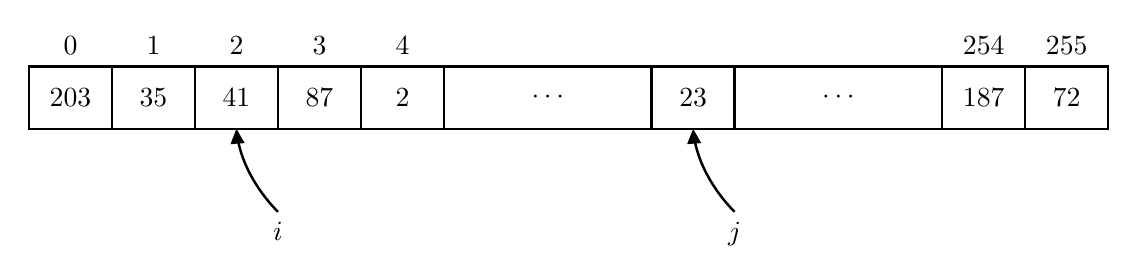
\begin{tikzpicture}[x=0.75pt,y=0.75pt,yscale=-1,xscale=1]
%uncomment if require: \path (0,125); %set diagram left start at 0, and has height of 125

%Shape: Rectangle [id:dp8774291212656176] 
\draw   (0,20) -- (520,20) -- (520,50) -- (0,50) -- cycle ;
%Straight Lines [id:da7417447618175568] 
\draw    (40,20) -- (40,50) ;
%Straight Lines [id:da7781155181250581] 
\draw    (80,20) -- (80,50) ;
%Straight Lines [id:da46532313693800553] 
\draw    (120,20) -- (120,50) ;
%Straight Lines [id:da891858566523396] 
\draw    (160,20) -- (160,50) ;
%Straight Lines [id:da9416263498656987] 
\draw    (200,20) -- (200,50) ;
%Straight Lines [id:da9145178928639244] 
\draw    (300,20) -- (300,50) ;
%Straight Lines [id:da9586008500216805] 
\draw    (340,20) -- (340,50) ;
%Straight Lines [id:da14035841668976134] 
\draw    (440,20) -- (440,50) ;
%Straight Lines [id:da2555764265900269] 
\draw    (480,20) -- (480,50) ;
%Curve Lines [id:da39731890421371974] 
\draw    (120,90) .. controls (112.82,82.82) and (102.51,69.12) .. (100.3,52.86) ;
\draw [shift={(100,50)}, rotate = 85.75] [fill={rgb, 255:red, 0; green, 0; blue, 0 }  ][line width=0.08]  [draw opacity=0] (7.14,-3.43) -- (0,0) -- (7.14,3.43) -- cycle    ;
%Curve Lines [id:da10312523213104918] 
\draw    (340,90) .. controls (332.82,82.82) and (322.51,69.12) .. (320.3,52.86) ;
\draw [shift={(320,50)}, rotate = 85.75] [fill={rgb, 255:red, 0; green, 0; blue, 0 }  ][line width=0.08]  [draw opacity=0] (7.14,-3.43) -- (0,0) -- (7.14,3.43) -- cycle    ;

% Text Node
\draw (20,35) node    {$203$};
% Text Node
\draw (60,35) node    {$35$};
% Text Node
\draw (100,35) node    {$41$};
% Text Node
\draw (140,35) node    {$87$};
% Text Node
\draw (180,35) node    {$2$};
% Text Node
\draw (250,35) node    {$\cdots $};
% Text Node
\draw (320,35) node    {$23$};
% Text Node
\draw (390,35) node    {$\cdots $};
% Text Node
\draw (460,35) node    {$187$};
% Text Node
\draw (500,35) node    {$72$};
% Text Node
\draw (20,10) node    {$0$};
% Text Node
\draw (60,10) node    {$1$};
% Text Node
\draw (100,10) node    {$2$};
% Text Node
\draw (140,10) node    {$3$};
% Text Node
\draw (180,10) node    {$4$};
% Text Node
\draw (460,10) node    {$254$};
% Text Node
\draw (500,10) node    {$255$};
% Text Node
\draw (120,93.4) node [anchor=north] [inner sep=0.75pt]    {$i$};
% Text Node
\draw (340,93.4) node [anchor=north] [inner sep=0.75pt]    {$j$};


\end{tikzpicture}